\documentclass[11pt]{article}

\usepackage[margin=1in]{geometry}
\usepackage{amsmath, amssymb, amsfonts}
\usepackage{bm}
\usepackage{graphicx}
\usepackage{enumitem}
\usepackage{tikz}
\usepackage{hyperref}

\title{General Stresses in Glaciers}
\author{Brent Minchew \\Caltech Ge 193, Spring 2026}
\date{}

\newcommand{\tens}[1]{\underline{\underline{#1}}}

\begin{document}

\maketitle

%===================================================================
% Topics Covered
%===================================================================
\section*{Topics Covered}

\begin{itemize}
  \item Review of forces, tractions, and the Cauchy stress tensor
  \item Symmetry of the stress tensor
  \item Principal stresses, principal axes, and stress invariants
  \item Decompositions of the stress tensor: deviatoric, isotropic, lithostatic, and non-lithostatic stress
\end{itemize}

\bigskip
\noindent \textbf{Primary reference:} Cuffey \& Paterson, \textit{Physics of Glaciers}, 4th ed.; supplemented by Malvern, \textit{Introduction to the Mechanics of a Continuous Medium}.

%===================================================================
% SECTION 1 -- Introduction
%===================================================================
\section{Introduction}

Glacier dynamics is, at its core, a problem in continuum mechanics: ice is a continuous medium that deforms under stress.  To understand how glaciers flow, we need a precise language for describing the forces that act within and upon the ice.  That language is the stress tensor.  In this lecture, we develop the mathematical framework for describing stress in a continuous body, prove key properties of the stress tensor, and introduce decompositions---deviatoric vs.\ isotropic, lithostatic vs.\ non-lithostatic---that will be essential when we derive the equations governing glacier flow in subsequent lectures.

\subsection*{Sign Convention}

A perennial source of confusion across mechanics: different communities use different sign conventions for stress.
\begin{itemize}
  \item \textbf{Tension-positive} (used in fluid mechanics, most of glaciology, and these notes): tensile (pulling apart) stresses are positive, compressive stresses are negative.
  \item \textbf{Compression-positive} (used in geology, rock mechanics, and some geodynamics): the opposite.
\end{itemize}
In these notes, we adopt the \textbf{tension-positive} convention throughout.  This means the lithostatic stress carries a negative sign ($\sigma_{ij}^{(L)} = -\rho_i g(s-z)\,\delta_{ij}$), because overburden is compressive.  When reading the glaciological literature, always check which convention an author uses---sign errors propagate silently and can reverse the physics.

%===================================================================
% SECTION 2 -- Review of Forces, Tractions, and Stress Tensors
%===================================================================
\section{Review of Forces, Tractions, and Stress Tensors}

\subsection{Forces and Tractions}
\begin{itemize}
  \item \textbf{Surface (a.k.a.\ contact) forces:} forces acting on a surface (i.e., forces resulting from a body acting on itself).
  \item \textbf{Body force:} forces that act throughout a volume and are due to external influences like gravity and mass.
  \item \textbf{Traction:} surface force that acts uniformly over a surface area; first-order tensor (i.e., vector).
        Can be decomposed into surface-normal and tangential (shear) components.
\end{itemize}

\subsection{The Cauchy Stress Tensor}
The (Cauchy, a.k.a.\ total) stress tensor is a 2\textsuperscript{nd}-order tensor that fully describes stresses at a point, i.e., a 2\textsuperscript{nd}-order tensor that specifies tractions on three mutually orthogonal faces of an infinitesimal cube.

\begin{figure}[ht]
\centering
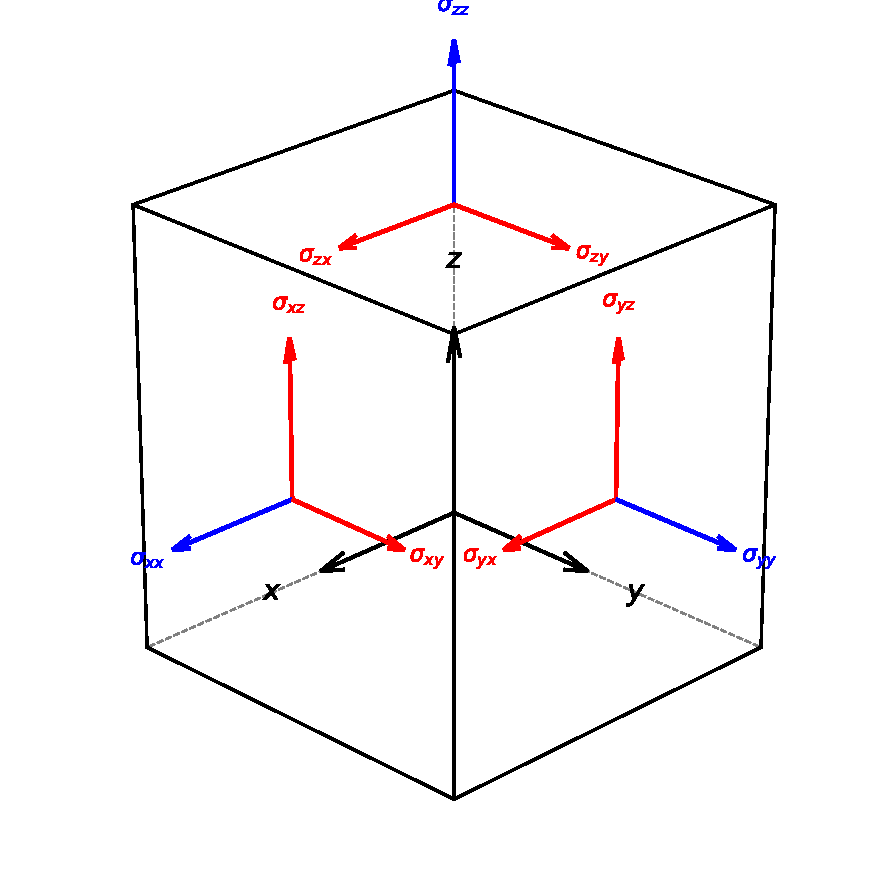
\includegraphics[width=0.55\textwidth]{stress_cube.pdf}
\caption{Components of the Cauchy stress tensor on an infinitesimal cube.  Normal stresses (blue) act perpendicular to each face; shear stresses (red) act tangentially.  Arrows are shown on the three positive faces ($+x$, $+y$, $+z$).  On a positive face, positive stress components point in the positive coordinate direction.}
\label{fig:stress_cube}
\end{figure}

\subsection{Cauchy's Formula}
Cauchy's formula relates tractions, stress tensors, and normals to arbitrary planes:
\begin{equation}
  T_i = \sigma_{ji}\, n_j \quad \left(\stackrel{\text{in most cases}}{=}\ \sigma_{ij}\, n_j\right)
\end{equation}

%===================================================================
% SECTION 3 -- Symmetry of the Stress Tensor
%===================================================================
\section{Symmetry of the Stress Tensor}

\textbf{Goal:} prove $\sigma_{ij} = \sigma_{ji}$ (in general).

To do so, we need to consider conservation of angular momentum---considering a body in equilibrium, the sum of moments (torques) about any point in a body must be zero.

\subsection{Setup: Moment Balance}

Consider a body of volume $V$ enclosed by surface $S$ (Fig.~\ref{fig:potato}).

\begin{figure}[ht]
\centering
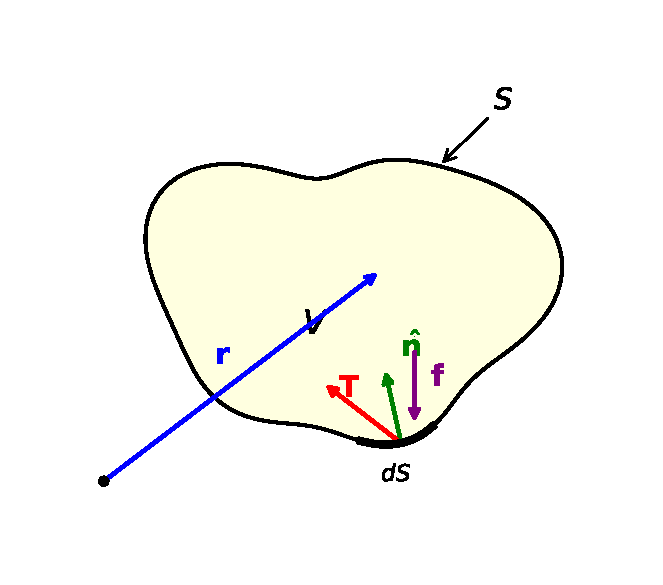
\includegraphics[width=0.45\textwidth]{potato_diagram.pdf}
\caption{An arbitrary body of volume $V$ bounded by surface $S$.  At a point on the surface, the traction $\bm{T}$ acts on a surface element $dS$ with outward normal $\hat{\bm{n}}$.  The body force $\bm{f}$ acts throughout the volume.  The position vector $\bm{r}$ is measured from the origin.}
\label{fig:potato}
\end{figure}

\noindent Define:
\begin{align*}
  \bm{r}   &= \text{position vector}  \\
  \bm{f}   &= \text{body force (per unit volume)}  \\
  \bm{T}   &= \text{traction}  \\
  \hat{\bm{n}}      &= \text{outward-pointing surface normal}
\end{align*}

\noindent Sum of moments:
\begin{equation}
  \bm{M} = \bm{0}
  = \int_S (\bm{r} \times \bm{T})\, dS
  + \int_V (\bm{r} \times \bm{f})\, dV
\end{equation}

\noindent Or in tensor notation:
\begin{equation}
  0 = \int_S \epsilon_{ijk}\, x_j\, T_k\, dS
    + \int_V \epsilon_{ijk}\, x_j\, f_k\, dV
\end{equation}
where $\epsilon_{ijk}$ is the Levi-Civita (permutation) symbol:
\[
  \epsilon_{ijk} =
  \begin{cases}
    +1 & \text{(even permutation), if } ijk = 123,\ 231,\ 312 \\
    -1 & \text{(odd permutation), if } ijk = 321,\ 213,\ 132 \\
    \phantom{+}0  & \text{otherwise (if any index is repeated)}
  \end{cases}
\]

Graphically, cycling $1 \to 2 \to 3 \to 1$ gives $+1$; cycling $1 \to 3 \to 2 \to 1$ gives $-1$.

\subsection{Proof}

Apply Cauchy's formula $T_i = \sigma_{ji}\, n_j$:
\begin{equation}
  0 = \int_S \epsilon_{ijk}\, x_j\, \sigma_{mk}\, n_m\, dS
    + \int_V \epsilon_{ijk}\, x_j\, f_k\, dV
\end{equation}

Apply the divergence theorem to convert the surface integral to a volume integral.

\begin{quote}
\textit{Divergence theorem} states that the outward flux of a tensor field through a closed surface equals the integral of the divergence over the volume inside the surface:
\[
  \int_S A_i\, n_i\, dS = \int_V A_{j,j}\, dV
\]
where $A_{j,j} = \nabla \cdot \bm{A}$ for an arbitrary tensor.
\end{quote}

\noindent The moment balance becomes:
\begin{equation}
  0 = \int_V \left(\epsilon_{ijk}\, x_j\, \sigma_{mk}\right)_{,m} dV
    + \int_V \epsilon_{ijk}\, x_j\, f_k\, dV
\end{equation}

Apply the chain rule and regroup:
\begin{equation}
  0 = \int_V \left(\epsilon_{ijk}\, \sigma_{mk}\, \delta_{jm}\right) dV
    + \int_V \epsilon_{ijk}\, x_j\, \underbrace{\left(\sigma_{mk,m} + f_k\right)}_{= 0\ \text{linear mom.}} dV
\end{equation}

The linear momentum term vanishes.  Applying the Kronecker delta and dropping the integral:
\begin{equation}
  \epsilon_{ijk}\, \sigma_{jk} = 0
\end{equation}

Applying the Levi-Civita symbol:
\begin{equation}
  \boxed{\sigma_{ij} = \sigma_{ji}} 
\end{equation}

%===================================================================
% SECTION 4 -- Principal Stresses and Stress Invariants
%===================================================================
\section{Principal Stresses and Stress Invariants}

\subsection{Principal Stresses and Principal Axes}

In general, the stress tensor represents tractions both perpendicular to the surface (i.e., normal tractions) and parallel to the surface (i.e., shear tractions).

But, in a certain coordinate system, the shear tractions vanish and only the nonzero components of the stress tensor are normal stresses.

$\Rightarrow$ These are the \textbf{principal stresses} and \textbf{principal axes} (or principal stress directions).

To see how this works, recall Cauchy's formula for the special case when all shear stresses are zero:
\begin{equation}
  T_i = \sigma_{ij}\, n_j = \lambda\, n_i
\end{equation}
where $\lambda$ is a scalar (0\textsuperscript{th}-order tensor).

Rearranging, we have
\begin{equation}
  (\sigma_{ij} - \lambda\, \delta_{ij})\, n_j = 0
  \qquad\quad \delta_{ij} \equiv \text{Kronecker delta}
\end{equation}

Expanding:
\begin{equation}
  \begin{bmatrix}
    \sigma_{xx} - \lambda & \sigma_{xy} & \sigma_{xz} \\
    \sigma_{xy} & \sigma_{yy} - \lambda & \sigma_{yz} \\
    \sigma_{xz} & \sigma_{yz} & \sigma_{zz} - \lambda
  \end{bmatrix}
  \begin{bmatrix} n_x \\ n_y \\ n_z \end{bmatrix}
  = \bm{0}
  \quad \Rightarrow \quad \text{eigenvalue problem}
\end{equation}

We know from linear algebra that this system of equations has a solution if
\begin{equation}
  \det\!\left(\sigma_{ij} - \lambda\, \delta_{ij}\right) = 0
\end{equation}

Expanding the determinant, we get
\begin{equation}
  \boxed{-\lambda^3 + \mathcal{I}_1\, \lambda^2 + \mathcal{I}_2\, \lambda + \mathcal{I}_3 = 0}
  \tag{1}
\end{equation}
where $\mathcal{I}_1$, $\mathcal{I}_2$, $\mathcal{I}_3$ are functions of the components of the stress tensor and are known as \textbf{stress invariants}.

(In fact, any 2\textsuperscript{nd}-order tensor that satisfies the characteristic equation above has invariants of the same form.)

\medskip

Eq.~(1) is a cubic equation $\Rightarrow$ has 3 solutions.  These are the magnitudes of the traction vector acting on each of the shear-free surfaces.

$\Rightarrow$ Solutions to Eq.~(1) are the \textbf{principal stresses}.

We denote the principal stresses $\sigma_1$, $\sigma_2$, $\sigma_3$.

Substituting these terms into the formula
\[
  \sigma_{ij}\, n_j = \lambda\, n_i \qquad \text{where } \lambda = \sigma_1,\, \sigma_2,\, \sigma_3
\]
we solve for eigenvectors $\hat{\bm{n}}_1$, $\hat{\bm{n}}_2$, $\hat{\bm{n}}_3$ $\to$ called \textbf{principal directions}.

We know from linear algebra that eigenvectors are mutually orthogonal $\Rightarrow$ the principal directions define a coordinate system, and these are the \textbf{principal axes}.

In the principal coordinates, we write the Cauchy stress tensor as
\begin{equation}
  \sigma_{ij} =
  \begin{bmatrix}
    \sigma_1 & 0 & 0 \\
    0 & \sigma_2 & 0 \\
    0 & 0 & \sigma_3
  \end{bmatrix}
\end{equation}

The 3 principal stresses are referred to by different terms, and herein lies a source of much confusion. It is important for you to pay attention to how terms are defined. 


\subsection{Why Do We Care About Principal Stresses?}

The main reason is that they are \textbf{invariant} under coordinate transform $\Rightarrow$ same in all coordinate systems.

$\Rightarrow$ Invariants are extremely valuable, as they uniquely define the stress state using only 3 values, independent of the coordinate system we choose.

\subsection{Stress Invariants}

Principal stresses are not the only invariants.

The terms $\mathcal{I}_1$, $\mathcal{I}_2$, $\mathcal{I}_3$ from Eq.~(1) must also be invariant if $\sigma_1$, $\sigma_2$, $\sigma_3$ are invariant.

$\mathcal{I}_1$, $\mathcal{I}_2$, $\mathcal{I}_3$ are usually called 1\textsuperscript{st}, 2\textsuperscript{nd}, 3\textsuperscript{rd} invariants for the stress tensor, defined as:
\begin{align}
  \mathcal{I}_1 &= \sigma_{kk} = \operatorname{tr}(\tens{\sigma})
                  = \text{trace of } \sigma_{ij} \\
  \mathcal{I}_2 &= \tfrac{1}{2}\!\left[(\sigma_{kk})^2 - \sigma_{ij}\,\sigma_{ij}\right]
                  = \tfrac{1}{2}\!\left[\left(\operatorname{tr}(\tens{\sigma})\right)^2
                    - \operatorname{tr}(\tens{\sigma}^2)\right] \\
  \mathcal{I}_3 &= \det(\tens{\sigma}) = \text{determinant of } \sigma_{ij}
\end{align}

We can also define invariants in terms of principal stresses:
\begin{align}
  \mathcal{I}_1 &= \sigma_1 + \sigma_2 + \sigma_3 \\
  \mathcal{I}_2 &= \sigma_1\,\sigma_2 + \sigma_2\,\sigma_3 + \sigma_3\,\sigma_1 \\
  \mathcal{I}_3 &= \sigma_1\,\sigma_2\,\sigma_3
\end{align}

\begin{itemize}
  \item Note the units on invariants.
  \item Further note on invariant usage: it is common in some fields (e.g., geodynamics) to refer to $\sqrt{\mathcal{I}_2}$ as the second invariant.
\end{itemize}

\subsection{Intuition for Invariants}

\begin{itemize}
  \item $\mathcal{I}_1 = \sigma_{kk}$ is proportional to the \textbf{mean normal stress} (i.e., pressure).  It captures the part of the stress state that tends to change the \emph{volume} of a material element without changing its shape.  Dividing by 3 gives the mean isotropic stress $p = \mathcal{I}_1/3$, which we will use to define the deviatoric stress tensor in Section~\ref{sec:decompositions}.

  \item $\mathcal{I}_2$ captures the \textbf{magnitude of shearing} in the stress state.  To see why, note that $\sigma_{ij}\sigma_{ij}$ (the squared Frobenius norm) measures the total ``size'' of the stress tensor, while $(\sigma_{kk})^2$ measures the volumetric part.  Their difference, $\mathcal{I}_2 = \tfrac{1}{2}[(\sigma_{kk})^2 - \sigma_{ij}\sigma_{ij}]$, isolates the shape-changing (deviatoric) contribution.  When we later define the deviatoric stress tensor $\tau_{ij}$, its second invariant $\mathcal{I}_2(\tau_{ij}) = \tau_{ij}\tau_{ij}/2$ becomes the basis for the \textbf{effective stress}---a single scalar that characterizes how intensely a material is being sheared.  This is the quantity that enters the flow law for ice.

  \item $\mathcal{I}_3 = \det(\sigma_{ij})$ characterizes the \textbf{mode of deformation}---whether the stress state is dominated by uniaxial tension, pure shear, or uniaxial compression.  We will not use it further in this course, but it appears in plasticity theory and failure criteria.
\end{itemize}

%===================================================================
% SECTION 5 -- Decompositions of the Stress Tensor
%===================================================================
\section{Decompositions of the Stress Tensor}
\label{sec:decompositions}

Recall that the Cauchy stress tensor is the complete representation of \textbf{total} stress at a point.

It is often desirable and useful to decompose the Cauchy stress tensor.  Two decompositions are particularly important in glacier dynamics: (1) deviatoric and isotropic stress, and (2) lithostatic and non-lithostatic stress.

\subsection{Deviatoric and Isotropic Stress}

The total stress at a point combines two physically distinct effects: stresses that change the \emph{volume} of a material element and stresses that change its \emph{shape}.  Separating these two contributions is useful in any material, but it is especially powerful in glaciology because the flow law for ice depends only on the shape-changing part.

We define the \textbf{mean isotropic stress} (often called ``pressure''):
\begin{equation}
  p = \frac{\mathcal{I}_1}{3} = \frac{\sigma_{kk}}{3}
\end{equation}

The \textbf{deviatoric stress tensor} is then defined as
\begin{equation}
  \boxed{\tau_{ij} = \sigma_{ij} - p\,\delta_{ij}}
\end{equation}

(You will also see the deviatoric stress tensor denoted $\sigma'_{ij}$, $\sigma_{ij}^{\text{dev}}$, or $s_{ij}$ in the literature.)

\subsubsection*{Why This Decomposition Matters for Glaciology}

\begin{itemize}
  \item \textbf{Ice deforms in response to deviatoric stress, not total stress.}  Glen's flow law---the constitutive relation for ice creep---relates the strain rate tensor to the deviatoric stress tensor:
  \begin{equation}
    \dot{\varepsilon}_{ij} = A\,\tau_e^{n-1}\,\tau_{ij}
  \end{equation}
  where $A$ is a rate factor (temperature-dependent), $n \approx 3$ is the creep exponent, and $\tau_e$ is the effective deviatoric stress (defined below).  The \textbf{strain rate tensor} $\dot{\varepsilon}_{ij}$ is the symmetric part of the velocity gradient:
  \begin{equation}
    \dot{\varepsilon}_{ij} = \frac{1}{2}\left(\frac{\partial u_i}{\partial x_j} + \frac{\partial u_j}{\partial x_i}\right)
  \end{equation}
  where $u_i$ is the $i$-th component of the ice velocity and $x_j$ is the $j$-th spatial coordinate.  Like the stress tensor, $\dot{\varepsilon}_{ij}$ is symmetric and can be decomposed into principal values and invariants.

  A fundamental constraint for glacier ice is \textbf{incompressibility}: ice does not change volume as it deforms, so the trace of the strain rate tensor vanishes:
  \begin{equation}
    \dot{\varepsilon}_{kk} = \frac{\partial u_x}{\partial x} + \frac{\partial u_y}{\partial y} + \frac{\partial u_z}{\partial z} = \bm{\nabla} \cdot \bm{u} = 0.
  \end{equation}
  This has two important consequences.  First, it means that pressure $p$ is not determined by the constitutive law---it enters only through the momentum equation and boundary conditions, acting as a Lagrange multiplier enforcing the volume constraint.  This is why Glen's flow law relates strain rate to \emph{deviatoric} stress alone, with no dependence on $p$.  Second, it reduces the number of independent strain rate components from six to five, just as tracelessness reduces the deviatoric stress tensor from six to five independent components.

  \item \textbf{Separates the ``interesting'' dynamics from the background pressure.}  Deep in a glacier, the total stress is dominated by the overburden pressure ($\sim \rho g h$), which can be tens of MPa.  The deviatoric stresses that actually drive flow are typically only $\sim$0.01--0.3~MPa---orders of magnitude smaller.  The decomposition isolates this small but dynamically important signal.
\end{itemize}

\textbf{Important:} $p = \sigma_{kk}/3$ is the mean of the normal stresses, not necessarily the hydrostatic or lithostatic pressure $\rho g h$.  The two coincide only when deviatoric normal stresses are negligible.

\subsubsection*{Properties of the Deviatoric Stress Tensor}

\begin{enumerate}
  \item Can have nonzero shear and normal stresses.
  \item Shear stresses are the same as in the Cauchy stress tensor: $\tau_{ij} = \sigma_{ij}$ for $i \neq j$.
  \item The deviatoric stress tensor is \textbf{traceless}:
    \begin{equation}
      \tau_{kk} = \mathcal{I}_1(\tau_{ij}) = 0
    \end{equation}
    This means the deviatoric tensor has only 5 independent components (not 6), because the three normal deviatoric stresses must sum to zero.
  \item The 2\textsuperscript{nd} invariant of $\tau_{ij}$ simplifies due to the traceless property:
    \begin{equation}
      \mathcal{I}_2(\tau_{ij}) = \frac{\tau_{ij}\,\tau_{ij}}{2}
    \end{equation}
\end{enumerate}

\subsubsection*{Effective Deviatoric Stress}

The \textbf{effective deviatoric stress} is the scalar
\begin{equation}
  \tau_e = \sqrt{\frac{\tau_{ij}\,\tau_{ij}}{2}} = \sqrt{\mathcal{I}_2(\tau_{ij})}
\end{equation}

This is the single number that enters Glen's flow law.  It represents the overall intensity of shearing at a point, regardless of the orientation of the coordinate system.  In glaciology, $\tau_e$ is sometimes called the ``effective stress'' or ``effective shear stress.''

\medskip
\noindent \textbf{Notation warning:} be cognizant of variable usage in the literature.  There are many conventions for distinguishing the Cauchy and deviatoric stress tensors, and notation varies between glaciology, geodynamics, and engineering.

\subsection{Lithostatic, Non-Lithostatic, and Resistive Stresses}

In a glacier, the dominant stress at any point is the weight of the overlying ice.  This motivates a second decomposition: removing the well-constrained gravitational contribution to isolate the stresses that resist or drive flow.

\subsubsection*{Lithostatic (Cryostatic) Stress}

The \textbf{lithostatic stress} (called \textbf{cryostatic} in glaciology, or \textbf{hydrostatic} in fluid mechanics) is the isotropic stress due to the overburden:
\begin{equation}
  \sigma_{ij}^{(L)} = -\rho_i g (s - z)\,\delta_{ij}
\end{equation}
where $s$ is the surface elevation, $z$ is the vertical coordinate (so $s - z$ is the depth below the surface), $\rho_i$ is the ice density, and $g$ is gravitational acceleration.  This is simply the pressure that would exist if the ice were a static fluid.

In a real glacier, the total stress differs from the cryostatic stress because of lateral pressure gradients, shearing, and longitudinal stretching or compression associated with flow.

\subsubsection*{Non-Lithostatic Stress}

The \textbf{non-lithostatic stress} removes the cryostatic contribution:
\begin{equation}
  \sigma_{ij}^{(nl)} = \sigma_{ij} - \sigma_{ij}^{(L)} = \sigma_{ij} + \rho_i g (s-z)\,\delta_{ij}
\end{equation}

\textbf{Advantage:} the cryostatic stress $\rho_i g(s-z)$ is known from the ice geometry alone---no knowledge of the flow field is needed.

\textbf{Disadvantage:} $\sigma_{ij}^{(nl)}$ mixes deviatoric and isotropic contributions, so it does not have as clean a physical interpretation as the deviatoric stress tensor.

\subsubsection*{Resistive Stresses}

In much of the glaciological literature, particularly following van der Veen \& Whillans (1989), the force balance is written in terms of \textbf{resistive stresses} $R_{ij}$, defined as
\begin{equation}
  \boxed{R_{ij} = \tau_{ij} + \delta_{ij}\,\rho_i g (s - z)}
\end{equation}
or equivalently $R_{ij} = \sigma_{ij} - \sigma_{ij}^{(L)} - (p + \rho_i g(s-z))\delta_{ij}$... but it is much clearer to think of it as: the full Cauchy stress with the cryostatic pressure removed, then further decomposed so that $R_{ij}$ inherits the deviatoric shear stresses but carries modified normal stresses.

In component form, the key resistive stresses are:
\begin{itemize}
  \item $R_{xx}$, $R_{yy}$: \textbf{longitudinal and transverse resistive stresses}---these resist or enhance longitudinal stretching/compression.  They equal the corresponding deviatoric normal stresses: $R_{xx} = 2\tau_{xx} + \tau_{yy}$, etc.\ (in the vertically integrated form).
  \item $R_{xy}$: \textbf{lateral shear resistive stress}---resists flow at the margins.  Equals $\tau_{xy}$.
  \item $R_{xz}$: \textbf{basal shear resistive stress}---resists flow at the bed.  Equals $\tau_{xz}$.
\end{itemize}

The resistive-stress formulation is useful because it expresses the depth-integrated force balance entirely in terms of quantities that can, in principle, be inferred from surface observations: surface slope (which sets the gravitational driving stress) and velocity gradients (which constrain the resistive stresses through the flow law).

\subsubsection*{Driving Stress}

The counterpart to resistive stress is the \textbf{gravitational driving stress}, which for a slab of ice on a slope with surface gradient $\partial s/\partial x$ is
\begin{equation}
  \tau_d = -\rho_i g h \frac{\partial s}{\partial x}
\end{equation}
where $h$ is the ice thickness.  In equilibrium, the driving stress is balanced by the sum of all resistive stresses (basal drag, lateral drag, and longitudinal stress gradients).  This balance is the starting point for most glacier flow models and will be derived formally in subsequent lectures.

\subsection{Distinguishing Deviatoric, Non-Lithostatic, and Resistive Stresses}

One of the most common conceptual errors in glaciology is conflating these three quantities.  To summarize:

\begin{itemize}
  \item \textbf{Deviatoric stress} $\tau_{ij} = \sigma_{ij} - p\,\delta_{ij}$, where $p = \sigma_{kk}/3$.  Physically separates shape-changing from volume-changing stresses.  Appears in the flow law.

  \item \textbf{Non-lithostatic stress} $\sigma_{ij}^{(nl)} = \sigma_{ij} + \rho_i g(s-z)\,\delta_{ij}$.  Removes the cryostatic pressure.  Easy to compute from geometry but mixes deviatoric and isotropic parts.

  \item \textbf{Resistive stress} $R_{ij}$: a hybrid that combines the deviatoric stress with the cryostatic correction.  Designed to make the depth-integrated force balance transparent.  Equals the deviatoric stress for shear components ($R_{xy} = \tau_{xy}$, $R_{xz} = \tau_{xz}$) but differs for normal components.
\end{itemize}

\medskip
\noindent\textbf{Key point:} $p = \sigma_{kk}/3$ is the mean of the normal stresses and is \emph{not} in general equal to $\rho_i g(s-z)$.  Referring to $p$ as ``hydrostatic pressure'' is a common error in the literature---avoid it.  The two coincide only when all deviatoric normal stresses vanish.

%===================================================================
% SECTION 6 -- Summary
%===================================================================
\section{Summary}

\begin{enumerate}
  \item The \textbf{Cauchy stress tensor} $\sigma_{ij}$ fully describes the state of stress at a point.  It is symmetric ($\sigma_{ij} = \sigma_{ji}$), which we proved from conservation of angular momentum.

  \item \textbf{Principal stresses} are the eigenvalues of $\sigma_{ij}$.  They are invariant under coordinate transformations, as are the stress invariants $\mathcal{I}_1$, $\mathcal{I}_2$, $\mathcal{I}_3$.

  \item The \textbf{deviatoric stress tensor} $\tau_{ij} = \sigma_{ij} - p\,\delta_{ij}$ separates shape-changing stresses from volume-changing stresses.  It is traceless and will appear throughout this course, particularly in the flow law for ice.

  \item Alternative decompositions sometimes appear in glaciology---do not confuse them:
  \begin{itemize}
    \item \textbf{Non-lithostatic stress} $\sigma_{ij}^{(nl)}$: total stress minus cryostatic pressure.
    \item \textbf{Resistive stress} $R_{ij}$: combines deviatoric stress with the cryostatic correction; makes the depth-integrated force balance transparent.
    \item Neither is the same as the deviatoric stress $\tau_{ij}$
   \end{itemize}

  \item The \textbf{driving stress} $\tau_d = -\rho_i g h\,\partial s/\partial x$ is balanced by resistive stresses (basal drag, lateral drag, longitudinal stress gradients)---the starting point for glacier flow models.
\end{enumerate}

\medskip
\noindent \textbf{Next:} conservation of linear momentum and the equations of motion for glacier ice.

%===================================================================
% Reading
%===================================================================
\section*{Reading}

Cuffey \& Paterson, \textit{Physics of Glaciers}, 4th ed.:
\begin{itemize}
  \item Section 8.2: Stress and strain rate (definitions, notation, and conventions for glacier mechanics)
  \item Section 8.3: Glen's flow law (constitutive relation, effective stress and strain rate)
  \item Section 8.4: Force balance (driving stress, resistive stresses, and the vertically integrated momentum equation)
\end{itemize}

\noindent Supplementary:
\begin{itemize}
  \item Malvern, \textit{Introduction to the Mechanics of a Continuous Medium}, Chapters 3--4: rigorous treatment of stress, principal stresses, and invariants.
  \item van der Veen \& Whillans (1989): the resistive-stress formulation used widely in glaciology.
  \item Glen (1955): the original experimental paper establishing the power-law creep relation for ice.
  \item Nye (1957): early application of plasticity theory to glacier flow, including the role of deviatoric stress.
\end{itemize}

%===================================================================
% Bibliography
%===================================================================
\begin{thebibliography}{99}

\bibitem{Glen1955}
Glen, J.~W.\ (1955).
The creep of polycrystalline ice.
\textit{Proceedings of the Royal Society of London.\ Series A}, 228(1175), 519--538.
\texttt{doi:10.1098/rspa.1955.0066}

\bibitem{Nye1957}
Nye, J.~F.\ (1957).
The distribution of stress and velocity in glaciers and ice-sheets.
\textit{Proceedings of the Royal Society of London.\ Series A}, 239(1216), 113--133.
\texttt{doi:10.1098/rspa.1957.0026}

\bibitem{vanderVeen1989}
van der Veen, C.~J.\ \& Whillans, I.~M.\ (1989).
Force budget: I.\ Theory and numerical methods.
\textit{Journal of Glaciology}, 35(119), 53--60.
\texttt{doi:10.3189/S0022143000004836}

\end{thebibliography}

\end{document}
